\newpage
\section{Chapter 2}

\begin{figure}[H]
	\centering
	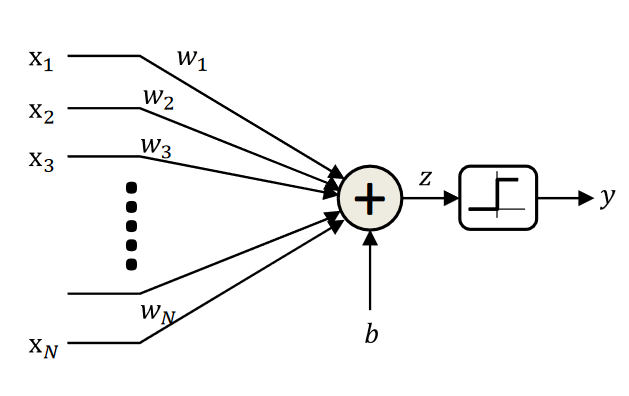
\includegraphics[width=0.5\textwidth]{2_perceptron}
\end{figure}

\hfill\break
Each individual neurons can be represented as a threshold unit.
\begin{itemize}
	\item It fires if the affine function of inputs is positive.
	\item The bias value is the negative of threshold $T$.
\end{itemize} 

\begin{align*}
	z &= \sum_{i}w_ix_i + b \\
	y &= 
\begin{cases} 
	1, & \text{if } z \geq 0 \\
	0, & \text{else }
\end{cases}
\end{align*}

\hfill\break
Once we can represent the neuron in this manner, we can modify the activation threshold function to something different such as:
\begin{itemize}
	\item We define \textbf{activation function} as the function that acts on the weighted combination of inputs and bias.
	 
\end{itemize}
\paragraph{Soft Perceptron (Logistic)}
A squashing function instead of a threshold at the output. This way the output goes rather smooth from $0$ to $1$.
\begin{align*}
	z &= \sum_{i}w_ix_i + b \\
	y &= \frac{1}{1 + \exp (-z)}
\end{align*}

\hfill\break
We can also replace the activation function with other mathematical function such as $\tanh$, $\text{softplus}$ and $\text{rectifier}$.

\subsection{Multi-layer Perceptron}
MLP is a network of perceptrons as the perceptrons of current layer are fed to other perceptrons on the next layer.

\paragraph{Deep Structures}
In any directed graph with input source nodes and output sink nodes, ``depth'' is the length of the longest path from a source to a sink.
\begin{itemize}
	\item A ``source'' node in a directed graph is a node that has only outgoing edges.
	\item A ``sink'' node is a node that has only incoming edges.
\end{itemize}

\hfill\break
This is an example of depth 2 graph.
\begin{figure}[H]
	\centering
	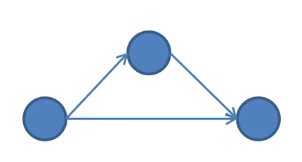
\includegraphics[width=0.4\textwidth]{2_2depth}
\end{figure}

\hfill\break
This is an example of depth 3 graph.
\begin{figure}[H]
	\centering
	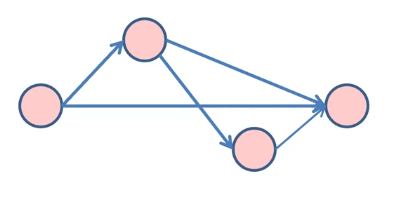
\includegraphics[width=0.4\textwidth]{2_3depth}
\end{figure}

\hfill\break
In multilayer perceptron, a network is considered ``deep'' if the depth of the output neurons is greater than $2$.

\subsection{Layer}
Layer is a set of neurons that are all at the same depth  with respect to the input (sink). This would imply that the ``depth'' of the layer is the depth of the neurons in the layer with respect to the input.

\begin{figure}[H]
	\centering
	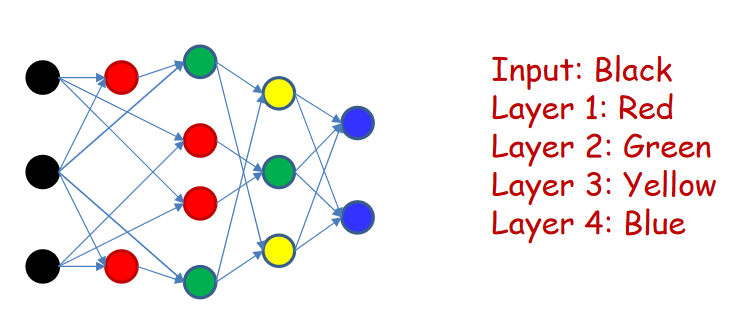
\includegraphics[width=0.75\textwidth]{2_layer}
\end{figure}

\hfill\break
In multi-layered perceptron:
\begin{itemize}
	\item Inputs are real or Boolean stimuli.
	\item Outputs are real or Boolean values.
	\item It can compose both Boolean and real-valued functions.
	\item We can have multiple outputs for a single input.
\end{itemize}

\subsection{MLP as universal Boolean functions.}
We are already aware with perceptron capability as a Boolean gate as it can model any simple binary Boolean gate (OR, AND \& NOT).

\begin{figure}[H]
	\centering
	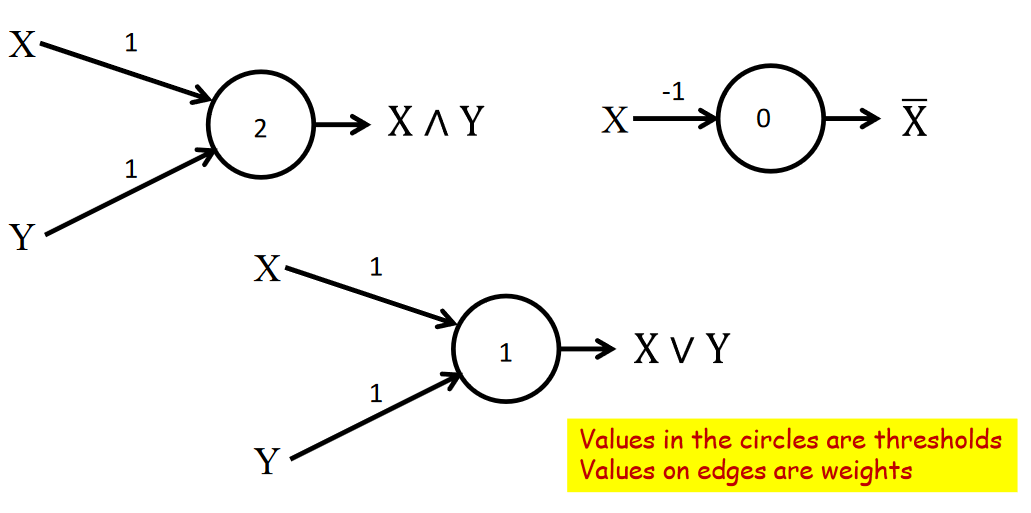
\includegraphics[width=\textwidth]{2_boolean_gate}
\end{figure}

\begin{itemize}
	\item For the AND gate, the boundary condition is $X + Y \geq 2$
	\item For the OR gate, the boundary condition is $X + Y \geq 1$
	\item For the NOT gate, the boundary condition is $-X \geq 0$
\end{itemize}

\hfill\break
It also enables us to compose a much more complex network, for example a universal AND gate where the network is only fired if every input fed to the network is true.

\paragraph{Universal AND Gate}

\begin{figure}[H]
	\centering
	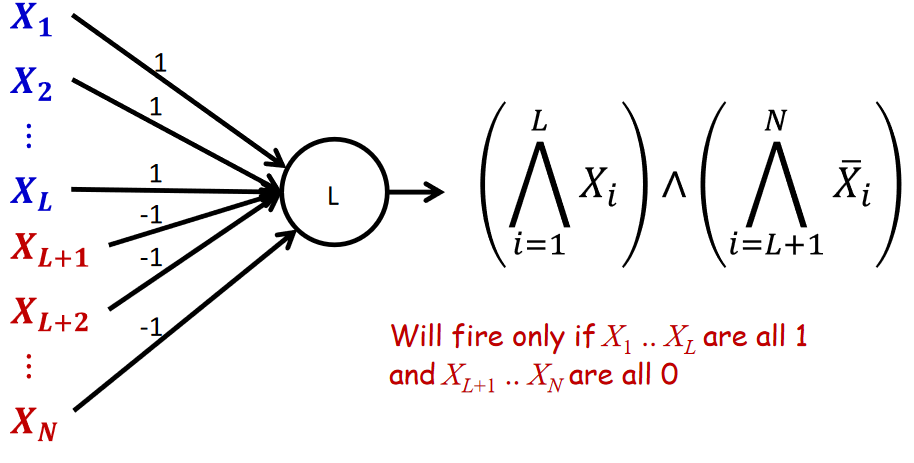
\includegraphics[width=0.5\textwidth]{2_universal_and}
\end{figure}

Suppose that $X_1,X_2,...,X_L$ has weight value of $1$ and $X_{L+1},X_{L+2},...,X_N$ has weight value of $-1$, the condition for the perceptron to fire has to be:
\begin{align}
	(X_1+X_2+...+X_L) - (X_{L+1},X_{L+2},...,X_N) \geq L
\end{align}

\paragraph{Universal OR Gate}

\begin{figure}[H]
	\centering
	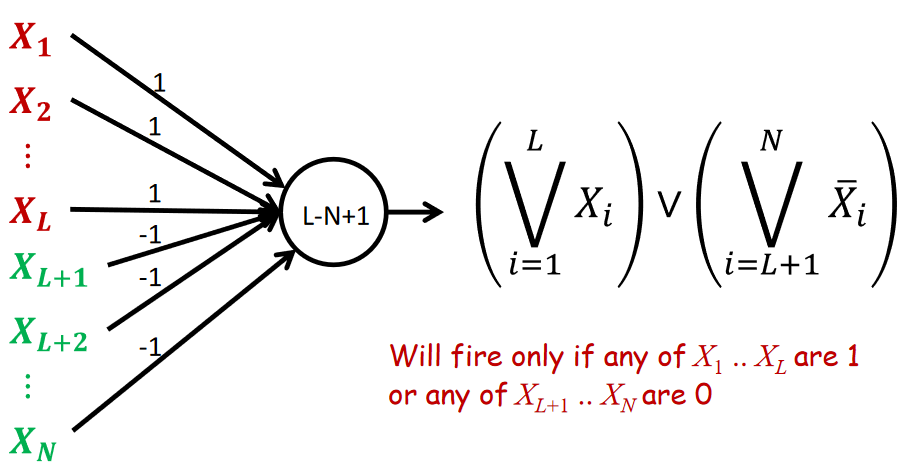
\includegraphics[width=0.5\textwidth]{2_universal_or}
\end{figure}

Suppose that $X_1,X_2,...,X_L$ has weight value of $1$ and $X_{L+1},X_{L+2},...,X_N$ has weight value of $-1$, the condition for the perceptron to fire has to be if any value of the first set is $1$ or any value from the second set is $0$:
\begin{align}
	(X_1+X_2+...+X_L) - (X_{L+1},X_{L+2},...,X_N) \geq L - N + 1
\end{align}

\paragraph{Generalized Majority Gate}

\begin{figure}[H]
	\centering
	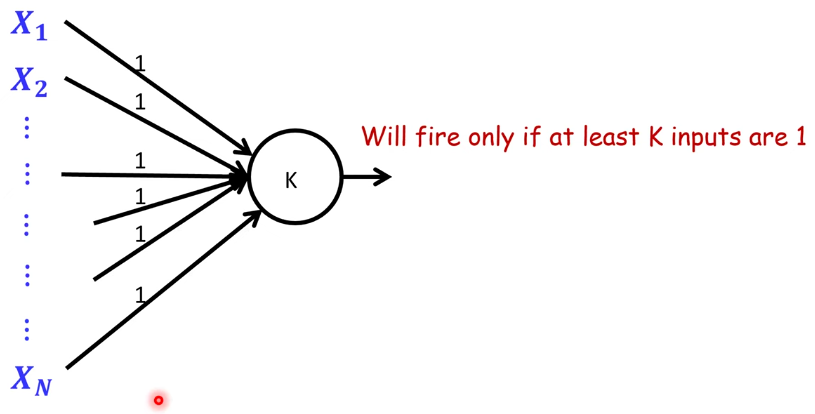
\includegraphics[width=0.5\textwidth]{2_majority_gate}
\end{figure}

\hfill\break
Due to perceptrons being able to model Boolean functions, they able to model complex things that are made of Boolean functions. This also means that for any odd Boolean function, wee can construct a multi-layerr perceptron that can compute this Boolean function. This is what is meant by MLPs being a universal Boolean functions. For any Boolean functions, regardless of their complexity, we can compose an MLP that will compute said function. This lead to a new question, how many layers will they need to be sufficient at modeling said Boolean function? What is the smallest number of layers will be required?


\hfill\break
Any Booleans function can be represented by a truth table. For example:


\begin{table}[H]
	\centering
	\begin{tabular}{|c|c|c|c|c|c|}
			\hline
			$X_1$    & $X_2$     & $X_3$    & $X_4$    & $X_5$    & $Y$   \\
			\hline
			0        & 0        & 1        & 1        & 0        & 1     \\
			0        & 1        & 0        & 1        & 1        & 1     \\
			0        & 1        & 1        & 0        & 0        & 1     \\
			1        & 0        & 0        & 0        & 1        & 1     \\
			1        & 0        & 1        & 1        & 1        & 1     \\
			1        & 1        & 0        & 0        & 1        & 1     \\
			\hline
	\end{tabular}
\end{table}

\hfill\break
In order to get a Boolean function that represent this table, we only have to list the portion of the table that corresponds to the output 1. We can write it as disjunctive normal formula for this table. 

\begin{align}
	Y = \bar{X_1}\bar{X_2}X_3X_4\bar{X_5} + \bar{X_1}X_2\bar{X_3}X_4X_5 + \bar{X_1}X_2X_3\bar{X_4}\bar{X_5} +\\ X_1\bar{X_2}\bar{X_3}\bar{X_4}X_5 + X_1\bar{X_2}X_3X_4X_5 + X_1X_2\bar{X_3}\bar{X_4}X_5
\end{align}

\hfill\break
Once we have obtained the Boolean function in this manner, we can create an MLP where each of the perceptron is an Universal AND gate. These perceptrons is then combined as Universal OR gate.


\begin{figure}[H]
	\centering
	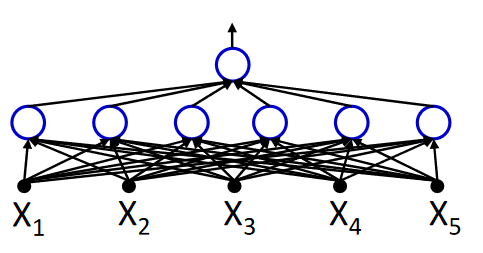
\includegraphics[width=0.5\textwidth]{2_truth_table}
\end{figure}

\hfill\break
This would means that MLP with 1 layer is sufficient enough to model any Boolean Function. This lead to a new question, what is the largest number of perceptrons required in the single hidden layer for an N-input-variable function?

\subsection{Karnaugh Map}
Boolean function can be reduced using Karnaugh Map. It represent a truth table as a grid. Adjacent boxes can be ``grouped'' to reduce the DNF formula for the table.

%\begin{figure}[H]
%\centering
%\begin{Karnaugh}{$v_w$}{$x_y$}
%	\content{0,0,0,0,0,0,0,0,0,0,0,0,0,0,0,0}
%	\implicant{0}{2}{red}
%	\implicant{5}{15}{purple}
%	\implicanttopbottom[3pt]{1}{10}{blue}
%	\implicantcorners[2pt]{orange}
%	\implicantside{4}{14}{green}
%\end{Karnaugh}
%\end{figure}

\begin{figure}[H]
	\centering
	\begin{Karnaugh}{$WX$}{$YZ$}
		\content{1,0,1,0,1,1,0,0,1,0,0,1,1,0,0,0}
	\end{Karnaugh}
\end{figure}







\subsection{Summary}
With enough ``depth'':
\begin{itemize}
	\item MLP as universal Boolean functions.
	\item MLP as universal classifiers.
	\item MLP as universal approximators.
\end{itemize}
